\documentclass[twocolumn]{article}
\usepackage[letterpaper, margin=1in]{geometry}
\usepackage{parskip}
\usepackage{fancybox}
\usepackage[table]{xcolor}
\usepackage{amsmath}
\usepackage{graphicx}
\usepackage[most]{tcolorbox}
\usepackage{makecell}

\usepackage{adjustbox}
\usepackage{titling}
\title{Project 3:\\Classification Using Neural Networks and Deep Learning}
\author{Youmi Koh}
\date{Sep 24, 2023}

\makeatletter
\def\@maketitle{
\newpage
 \null
 \vskip 0em
 \begin{center}
  {\Large \@title \par}%
 \end{center}%
 \vskip 1.8em}
\makeatother

\usepackage{fancyhdr}
\fancypagestyle{plain}{
    \fancyhf{}
    \fancyhead[L]{CSE575 - Sep 30, 2023}
    \fancyhead[R]{Youmi Koh - ID:1231025486}
}

\makeatletter
\renewcommand{\verbatim@font}{\scriptsize\ttfamily}
\makeatother


\newcolumntype{C}{>{\ttfamily\footnotesize}c}

\begin{document}
\maketitle
\noindent


\subsection*{Experiments with Baseline}

Baseline parameters consisted of the first layer with 3$\times$3 kernel size and 6 feature maps, and the second layer with 3$\times$3 kernel size and 16 feature maps. Then kernel size was modified\footnote{Please see \texttt{colab\_baseline.ipynb} code file for direct references to the project overview required tasks} to 5$\times$5 from 3$\times$3 and the number of feature maps to 6 in the first and second convolution layers. The following are results from training over 10 epochs:

\begin{table}[h]
    \centering
    \begin{tabular}{|C|C|C|}
        \hline
        Experiment
                 & Test Loss & Test Accuracy \\ \hline \hline
        Baseline & 0.0677    & 0.9786        \\ \hline
        \makecell{5x5 Kernel Size            \\ (Layer 1)}& 0.0573 & 0.9811  \\ \hline
        \makecell{5x5 Kernel Size            \\ (Layer 1\&2)}& 0.0605 & 0.9815  \\ \hline
        \makecell{6 Feature Maps             \\ (Layer 1\&2)}& 0.0842 & 0.9734 \\ \hline
    \end{tabular}
\end{table}

\begin{figure}[h]
    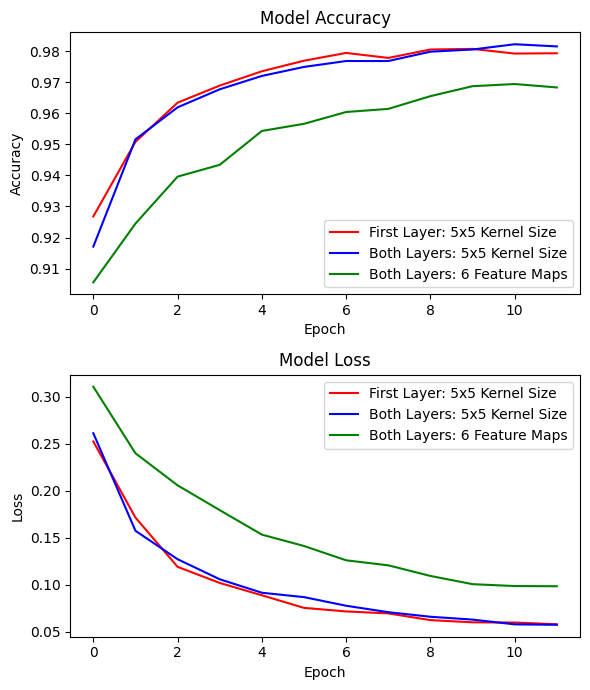
\includegraphics[width=0.46\textwidth]{baseline-plots.png}
\end{figure}

Increasing the kernel size on the first layer allows the model to capture more spatial information and the results show an improvement to test loss and test accuracy. When the kernel size is increased to the second layer, the results show an similarly expected improvement in test accuracy (albeit small) but also a slight increase to test loss. While likely insignificant, it may signal a shift in bias-variance tradeoff where the increased kernel size reduced bias (increasing test accuracy) but increased variance (increasing test loss).

The final experiment was to set the number of feature maps to 6 for both convolution layers. Since layer 1 was already set to 6 feature maps, this experiment only decreased the number of feature maps for layer to from 16 to 6. This resulted in a decrease in test accuracy and an increase in test loss. This is likely due to the model's reduced capacity to learn complex features leading to underfitting.

\subsection*{Results from CNN Train/Test Lab}

\begin{verbatim}
Train Acc:0.821, Train Loss:0.510, Test Acc:0.755, Test Loss:0.652
\end{verbatim}

\subsection*{\texttt{evaluate()} function from lab session}

To evaluate the model, the \texttt{evaluate()} function was implemented to calculate the accuracy and loss of the model. It first initializes the accuracy and loss to 0, then iterates over the images in batches of size 1 and performs a forward pass through the network. The output of the network is then compared to the label to calculate the loss and accuracy using cross entropy. Final loss/accuracy values normalized by dividing by the number of samples.

\begin{verbatim}
def evaluate(net, images, labels):
    # Initialize accuracy and loss to 0
    acc = 0
    loss = 0

    # Set batch size to 1 for evaluation
    batch_size = 1

    # Iterate over the images in batches
    for batch_index in range(0, images.shape[0], batch_size):
        # Select the current batch of images and labels
        if batch_index + batch_size < images.shape[0]:
            data = images[batch_index : batch_index + batch_size]
            label = labels[batch_index : batch_index + batch_size]
        else:
            data = images[batch_index : images.shape[0]]
            label = labels[batch_index : labels.shape[0]]

        # Forward pass through the network
        x, y = data[0], label[0]
        for l in range(net.lay_num):
            output = net.layers[l].forward(x)
            x = output

        # Calculate loss using cross entropy
        loss += cross_entropy(output, y)

        # Update accuracy if the prediction is correct
        if np.argmax(output) == np.argmax(y):
            acc += 1

    return acc / images.shape[0], loss / images.shape[0]
\end{verbatim}

\newpage
\subsection*{Plots from lab session}

\begin{figure}[h]
    \centering
    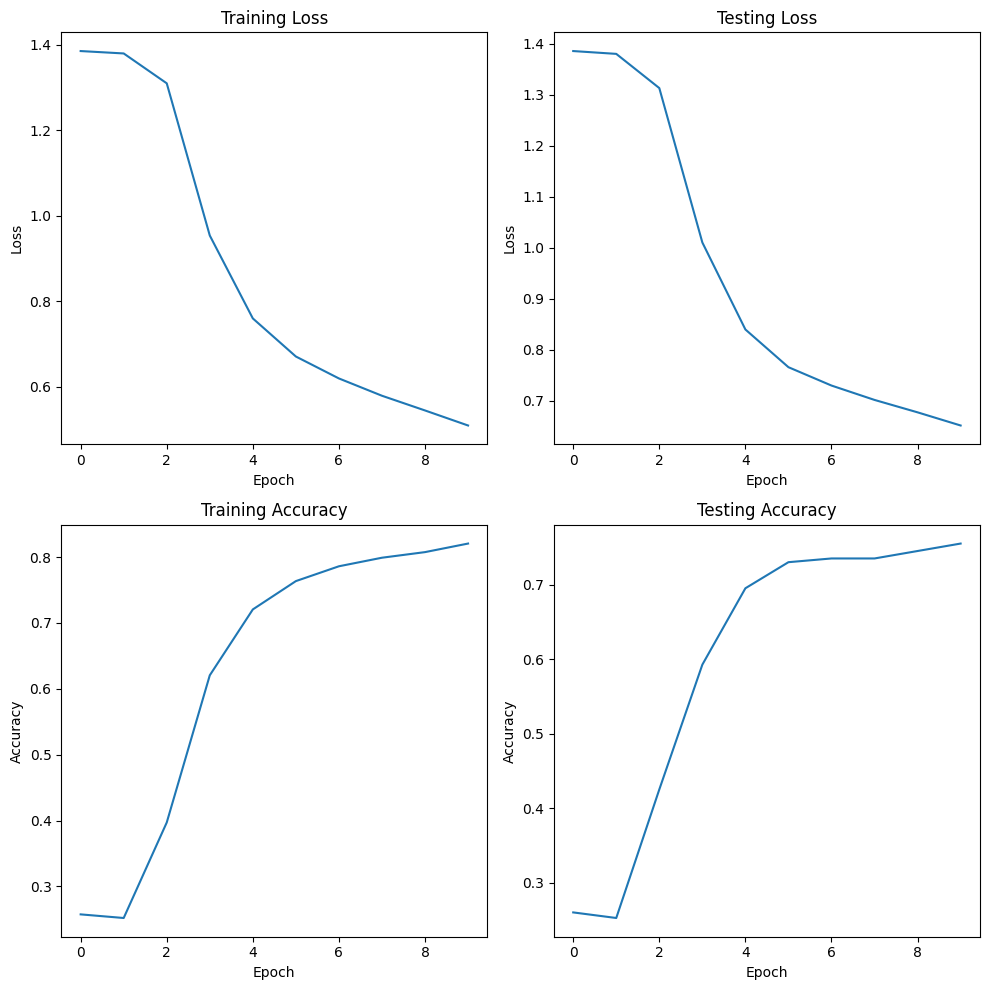
\includegraphics[width=1\textwidth]{lab-plots.png}
\end{figure}



\end{document}
